\documentclass{article}

\title{Audio Engineering Considerations for a Modern Mixnet}
\author{Brett Alexander Preston}
\date{October 2023}

\usepackage[T1]{fontenc}
%\usepackage[latin9]{inputenc}
\usepackage{geometry}
\geometry{verbose,tmargin=2.25cm,bmargin=2.25cm,lmargin=2.25cm,rmargin=2.5cm}
\usepackage{setspace}
%\onehalfspacing
\usepackage{babel}
\usepackage[table]{xcolor}
\usepackage{graphicx}
\usepackage{subfigure, wrapfig}
\usepackage{amssymb, amsmath}
\usepackage{tikz}
\usepackage{epsdice}
\clubpenalty=10000
\widowpenalty=10000
\usepackage{hyperref}
\setcounter{tocdepth}{3}
\usepackage{tabularx}
%\usepackage[square,numbers]{natbib}

\definecolor{blue}{HTML}{008ED7}
\definecolor{lightBlue}{HTML}{e5f7ff}
\newcommand{\n}{\cellcolor{green!10} not capable}
\newcommand{\y}{\cellcolor{purple!10} capable}
\begin{document}

\maketitle

\begin{center}
This work was supported by a grant from the Wau Holland Foundation.
\end{center}\medskip

\noindent Privacy-enhancing technologies have always faced a challenge in balancing security guarantees with user experience that would bring people to the service. In the contemporary communication landscape, most users expect their messengers to allow for some form of audio communication. We would therefore like to meet that demand without compromising anonymity.

The most ambitious private messengers being built today are those based on modern Mixnet designs. They introduce padding, in addition to a network of relays, and have to contend with latency. They distinguish themselves by considering realistic powerful adversaries and endeavoring to protect both the content of the communication and the metadata. This turns out to be crucial in the case of audio communication, since in most common implementations the metadata leaks content, so you can't have one without the other. We will therefore discuss implementation recommendations from an audio engineering point of view in adding audio communication to a Mixnet. We will look at how we can balance efficiency and user experience in this unique setting while upholding security guarantees.

\tableofcontents
\medskip

A modern Mixnet typically uses padding in order to mitigate traffic analysis. \cite{loopix} This means that a constant amount of traffic is being sent by a user at all times. The amount of traffic it allows for is also an upper limit to how much data a user can send. It is not realistic to set this limit too high, since it would quickly add up to a significant drain on a  user's resources. Therefore we should expect any audio communication to either have to be compressed to a low bitrate, or take a long time to travel through the network, which can make real-time audio communication impossible. %At the end of the day, you want non real-time communication. It provides better efficiency and limits the attack surface. 
Therefore we will consider non-synchronous push-to-talk messaging as an important mode of audio communication in this setting.

\pagebreak
\section{Content leaks in common encrypted VoIP implementations}
It has been demonstrated that encrypted real-time VoIP communications can produce devastating data leaks by not accounting for the fact that different phonemes are connected to different bitrates. Already in 2011, researchers were able to reconstruct sections of conversations from encrypted connections based on packet traffic patterns alone. \cite{phonemes}  Today, the threat is even more dire due to increased prevalence of Machine Learning and therefore the automation of powerful statistical analysis. \cite{phonemesdl} And yet popular communication software does not address this.

One can typically mitigate this problem by either using constant bit-rate encoding, therefore increasing the overall file size, or opting for push-to-talk messaging instead of real-time communication, where you process the entire recording. This goes back to the Anonymity Trilemma \cite{trilemma}: to maintain security guarantees, you have to compromise either on the overhead or on latency. But a Mixnet with padding has already made these compromises and so it faces these challenges by design.

\section{Recommendations for audio encoding and decoding}

Encoding and decoding  audio in a Mixnet has a unique set of challenges. We are particularly interested in efficiency, as there may be a strict bandwidth limit, but at the same time we have access to the computing power of a modern device and modern audio encoding and decoding tricks. We can reasonably expect to deal with some latency, and depending on the transport-layer protocol used we may have to consider some packet loss. We can also expect a modern Mixnet to prioritize security and to require its components to use licensing that supports freedom.

We will assume that padding and/or non-synchronicity allow for an implementation of VBR encoding without leaking content. We should still keep in mind security risks that come from haphazard implementations of VBR decoding, as sometimes they might allow for injection of malicious code. We should make sure the decoder we're using has been audited. An example of a decoder written with security in mind is Rust-based Symphonia \cite{symphonia}.

The following table is a comparison of file sizes in kBs generated by VBR encoding in various codecs, starting with a lossless wav file. The cells are clickable, so the reader can verify the sound quality. For the HTML version of this table, visit \href{https://brettpreston.github.io/mixnet-samples}{https://brettpreston.github.io/mixnet-samples}.


\begin{center}
\begin{table}
\fontfamily{cmss}\selectfont
\begin{tabularx}{\textwidth}[t]{| m{0.1\textwidth}| m{0.07\textwidth} |  m{0.08\textwidth}| m{0.09\textwidth}| m{0.07\textwidth}| m{0.075\textwidth}| m{0.08\textwidth}| m{0.1\textwidth}| m{0.1\textwidth}| }
\arrayrulecolor{gray}\hline 
\rowcolor{gray!20} 
        Codec & Bitrate & Frequency band width & Complexity & Deep voice (32sec) & Deep voice + noise 35 sec & High Voice & High voice+noise 49 sec & Generic rock 51 sec \\ \hline
        wav & ~ & ~ & ~ & \href{https://brettpreston.github.io/audio/KnPAudio/wav/deep-voice.wav} {2930} & \href{https://brettpreston.github.io/audio/KnPAudio/wav/deep-voice-noise.wav} {2990}  & \href{https://brettpreston.github.io/audio/KnPAudio/wav/high-voice.wav} {4560} & \href{https://brettpreston.github.io/audio/KnPAudio/wav/high-voice-noise.wav} {4330} & \href{https://brettpreston.github.io/audio/KnPAudio/wav/generic-rock.wav} {6620} \\ \hline
        opus & 64 kbps & wide & 10 & \href{https://brettpreston.github.io/audio/KnPAudio/opus/64vbr-wide-10cmplx/deep-voice.opus}{304} & \href{https://brettpreston.github.io/audio/KnPAudio/opus/64vbr-wide-10cmplx/deep-voice-noise.opus}{271} & \href{https://brettpreston.github.io/audio/KnPAudio/opus/64vbr-wide-10cmplx/high-voice.opus}{456} & \href{https://brettpreston.github.io/audio/KnPAudio/opus/64vbr-wide-10cmplx/high-voice-noise.opus}{390} & \href{https://brettpreston.github.io/audio/KnPAudio/opus/64vbr-wide-10cmplx/generic-rock.opus}{293} \\ \hline
        opus & 32 kbps & wide & 10 & \href{https://brettpreston.github.io/audio/KnPAudio/opus/32vbr-wide-10cmplx/deep-voice.opus}{113} & \href{https://brettpreston.github.io/audio/KnPAudio/opus/32vbr-wide-10cmplx/deep-voice-noise.opus}{131} & \href{https://brettpreston.github.io/audio/KnPAudio/opus/32vbr-wide-10cmplx/high-voice.opus}{170} & \href{https://brettpreston.github.io/audio/KnPAudio/opus/32vbr-wide-10cmplx/high-voice-noise.opus}{190} & \href{https://brettpreston.github.io/audio/KnPAudio/opus/32vbr-wide-10cmplx/generic-rock.opus}{137} \\ \hline
        opus & 16 kbps & wide & 10 & \href{https://brettpreston.github.io/audio/KnPAudio/opus/16vbr-wide-10cmplx/deep-voice.opus}{59.1} & \href{https://brettpreston.github.io/audio/KnPAudio/opus/16vbr-wide-10cmplx/deep-voice-noise.opus}{68.5} & \href{https://brettpreston.github.io/audio/KnPAudio/opus/16vbr-wide-10cmplx/high-voice.opus}{89.7} & \href{https://brettpreston.github.io/audio/KnPAudio/opus/16vbr-wide-10cmplx/high-voice-noise.opus}{98.4} & \href{https://brettpreston.github.io/audio/KnPAudio/opus/16vbr-wide-10cmplx/generic-rock.opus}{71.6} \\ \hline
        opus & 12 kbps & wide & 10 & \href{https://brettpreston.github.io/audio/KnPAudio/opus/12vbr-wide-10cmplx/deep-voice.opus}{45.4} & \href{https://brettpreston.github.io/audio/KnPAudio/opus/12vbr-wide-10cmplx/deep-voice-noise.opus}{51.8} & \href{https://brettpreston.github.io/audio/KnPAudio/opus/12vbr-wide-10cmplx/high-voice.opus}{69.4} & \href{https://brettpreston.github.io/audio/KnPAudio/opus/12vbr-wide-10cmplx/high-voice-noise.opus}{74.7} & \href{https://brettpreston.github.io/audio/KnPAudio/opus/12vbr-wide-10cmplx/generic-rock.opus}{54.5} \\ \hline
        opus & 12 kbps & wide & 5 & \href{https://brettpreston.github.io/audio/KnPAudio/opus/12vbr-wide-5cmplx/deep-voice.opus}{45} & \href{https://brettpreston.github.io/audio/KnPAudio/opus/12vbr-wide-5cmplx/deep-voice-noise.opus}{50.4} & \href{https://brettpreston.github.io/audio/KnPAudio/opus/12vbr-wide-5cmplx/high-voice.opus}{68.4} & \href{https://brettpreston.github.io/audio/KnPAudio/opus/12vbr-wide-5cmplx/high-voice-noise.opus}{72.5} & \href{https://brettpreston.github.io/audio/KnPAudio/opus/12vbr-wide-5cmplx/generic-rock.opus}{53.5} \\ \hline
        opus & 12 kbps & narrow & 5 & \href{https://brettpreston.github.io/audio/KnPAudio/opus/12vbr-narrow-5cmplx/deep-voice.opus}{49} & \href{https://brettpreston.github.io/audio/KnPAudio/opus/12vbr-narrow-5cmplx/deep-voice-noise.opus}{54.5} & \href{https://brettpreston.github.io/audio/KnPAudio/opus/12vbr-narrow-5cmplx/high-voice.opus}{76.2} & \href{https://brettpreston.github.io/audio/KnPAudio/opus/12vbr-narrow-5cmplx/high-voice-noise.opus}{78.6} & \href{https://brettpreston.github.io/audio/KnPAudio/opus/12vbr-narrow-5cmplx/generic-rock.opus}{60.2} \\ \hline
        opus & 6 kbps & wide & 10 & \href{https://brettpreston.github.io/audio/KnPAudio/opus/6vbr-wide-10cmplx/deep-voice.opus}{25.9} & \href{https://brettpreston.github.io/audio/KnPAudio/opus/6vbr-wide-10cmplx/deep-voice-noise.opus}{26.9} & \href{https://brettpreston.github.io/audio/KnPAudio/opus/6vbr-wide-10cmplx/high-voice.opus}{41} & \href{https://brettpreston.github.io/audio/KnPAudio/opus/6vbr-wide-10cmplx/high-voice-noise.opus}{39.3} & \href{https://brettpreston.github.io/audio/KnPAudio/opus/6vbr-wide-10cmplx/generic-rock.opus}{30.6} \\ \hline
        opus & 6 kbps & wide & 5 & \href{https://brettpreston.github.io/audio/KnPAudio/opus/6vbr-wide-5cmplx/deep-voice.opus}{25.6} & \href{https://brettpreston.github.io/audio/KnPAudio/opus/6vbr-wide-5cmplx/deep-voice-noise.opus}{26.4} & \href{https://brettpreston.github.io/audio/KnPAudio/opus/6vbr-wide-5cmplx/high-voice.opus}{40.1} & \href{https://brettpreston.github.io/audio/KnPAudio/opus/6vbr-wide-5cmplx/high-voice-noise.opus}{38.6} & \href{https://brettpreston.github.io/audio/KnPAudio/opus/6vbr-wide-5cmplx/generic-rock.opus}{30.2} \\ \hline                
        opus & 6 kbps & narrow & 5 & \href{https://brettpreston.github.io/audio/KnPAudio/opus/6vbr-narrow-5cmplx/deep-voice.opus}{25.4} & \href{https://brettpreston.github.io/audio/KnPAudio/opus/6vbr-narrow-5cmplx/deep-voice-noise.opus}{28.2} & \href{https://brettpreston.github.io/audio/KnPAudio/opus/6vbr-narrow-5cmplx/high-voice.opus}{36.4} & \href{https://brettpreston.github.io/audio/KnPAudio/opus/6vbr-narrow-5cmplx/high-voice-noise.opus}{40.7} & \href{https://brettpreston.github.io/audio/KnPAudio/opus/6vbr-narrow-5cmplx/generic-rock.opus}{31.2} \\ \hline       
        speex & 64 kbps & wide & 10 & \href{https://brettpreston.github.io/audio/KnPAudio/speex/64vbr-wide-10cmplx/deep-voice.spx}{165} & \href{https://brettpreston.github.io/audio/KnPAudio/speex/64vbr-wide-10cmplx/deep-voice-noise.spx}{166} & \href{https://brettpreston.github.io/audio/KnPAudio/speex/64vbr-wide-10cmplx/high-voice.spx}{256} & \href{https://brettpreston.github.io/audio/KnPAudio/speex/64vbr-wide-10cmplx/high-voice-noise.spx}{242} & \href{https://brettpreston.github.io/audio/KnPAudio/speex/64vbr-wide-10cmplx/generic-rock.spx}{126} \\ \hline
        speex & 32 kbps & wide & 10 & \href{https://brettpreston.github.io/audio/KnPAudio/speex/32vbr-wide-10cmplx/deep-voice.spx}{95.2} & \href{https://brettpreston.github.io/audio/KnPAudio/speex/32vbr-wide-10cmplx/deep-voice-noise.spx}{109} & \href{https://brettpreston.github.io/audio/KnPAudio/speex/32vbr-wide-10cmplx/high-voice.spx}{145} & \href{https://brettpreston.github.io/audio/KnPAudio/speex/32vbr-wide-10cmplx/high-voice-noise.spx}{158} & \href{https://brettpreston.github.io/audio/KnPAudio/speex/32vbr-wide-10cmplx/generic-rock.spx}{108} \\ \hline
        speex & 12 kbps & wide & 10 & \href{https://brettpreston.github.io/audio/KnPAudio/speex/12vbr-wide-10cmplx/deep-voice.spx}{36.3} & \href{https://brettpreston.github.io/audio/KnPAudio/speex/12vbr-wide-10cmplx/deep-voice-noise.spx}{42.4} & \href{https://brettpreston.github.io/audio/KnPAudio/speex/12vbr-wide-10cmplx/high-voice.spx}{55.7} & \href{https://brettpreston.github.io/audio/KnPAudio/speex/12vbr-wide-10cmplx/high-voice-noise.spx}{51.1} & \href{https://brettpreston.github.io/audio/KnPAudio/speex/12vbr-wide-10cmplx/generic-rock.spx}{54.3} \\ \hline
        speex & 4 kbps & wide & 10 & \href{https://brettpreston.github.io/audio/KnPAudio/speex/4vbr-wide-10cmplx/deep-voice.spx}{22.5} & \href{https://brettpreston.github.io/audio/KnPAudio/speex/4vbr-wide-10cmplx/deep-voice-noise.spx}{25} & \href{https://brettpreston.github.io/audio/KnPAudio/speex/4vbr-wide-10cmplx/high-voice.spx}{34.9} & \href{https://brettpreston.github.io/audio/KnPAudio/speex/4vbr-wide-10cmplx/high-voice-noise.spx}{36} & \href{https://brettpreston.github.io/audio/KnPAudio/speex/4vbr-wide-10cmplx/generic-rock.spx}{35.3} \\ \hline
        codec2 & 3200bps & default & n/a & \href{https://brettpreston.github.io/audio/KnPAudio/codec2/deep-voice-3200.c2.flac}{12.7} & \href{https://brettpreston.github.io/audio/KnPAudio/codec2/deep-voice-noise-3200.c2.flac}{14.1} & \href{https://brettpreston.github.io/audio/KnPAudio/codec2/high-voice-3200.c2.flac}{19.9} & \href{https://brettpreston.github.io/audio/KnPAudio/codec2/high-voice-noise-3200.c2.flac}{20.4} & \href{https://brettpreston.github.io/audio/KnPAudio/codec2/generic-rock-3200.c2.flac}{15.5} \\ \hline
        codec2 & 1200bps & default & n/a & \href{https://brettpreston.github.io/audio/KnPAudio/codec2/deep-voice-1200.c2.flac}{4.74} & f & \href{https://brettpreston.github.io/audio/KnPAudio/codec2/high-voice-1200.c2.flac}{7.47} & f & f \\ \hline
        codec2 & 450bps & default & n/a & \href{https://brettpreston.github.io/audio/KnPAudio/codec2/deep-voice-450.c2.flac}{2.4} & f & \href{https://brettpreston.github.io/audio/KnPAudio/codec2/high-voice-450.c2.flac}{3.73} & f & f \\ 
\arrayrulecolor{gray}
\hline
\end{tabularx}
\end{table}
\end{center}
\newpage

The key takeaways from this table can be summarized as follows. Opus delivers the best quality of the three codecs, and is the only one that can handle more than speech. With Opus we observe diminishing returns with quality above 12 kbps. Frequency band width has a small impact on the file size. Algorithm complexity has negligible impact on the file size, it primarily impacts local processing requirements. Codec2 delivers very, very small file size but can't handle noise or music at all. We go into detail on all of these points below.



\subsection{Audio codecs}

We have selected audio codecs that can be candidates for use in this setting. They deliver either impressive sound quality at low bitrates, or good sound quality and impressively low bitrates, and each has different strengths. Opus and Speex are under a BSD license, and Codec2 under LGPL.


\subsubsection*{Opus and Speex}

By far the most popular codec today, Opus is used in most modern VoIP systems. It is a versatile audio codec that is known for its high-quality, crisp sound reproduction, suitable for a wide range of applications, including voice communication and music streaming. It has ready implementations in many programming languages, including Go \cite{pion} and Rust \cite{symphonia}. It is also well documented, simplifying its potential integration into various projects. \cite{opusdoc}

Another fine codec for speech compression is Speex, which was popular in VoIP systems before the rise of Opus. It delivers clear and bright speech, but is not meant to be used for other sound. There are extensive resources which compare Opus to Speex \cite{opuscomp} \cite{opuscomp2}, and it is clear that Opus is both more efficient and more versatile.
\subsubsection*{Codec2}

For this special use case of Mixnets, we may also consider Codec2 because it is capable of extremely efficient encoding. Its efficiency relies heavily on sinusoidal coding and a narrow frequency band, which means that we quickly lose clarity and some distinguishing features of the original speech recording. The simplified harmonic content encodes less information compared to the popular codecs. 

However, in this particular context both the extremely small file size and the voice masking\footnote{Voice masking should not be treated as a guarantee of voice anonymity.} provided by the loss of distinguishing features may be desirable. It appears that Codec2 was originally intended for radio broadcast, in which case some of its shortcomings would be somewhat mitigated by post processing typically used for radio broadcast.
If we were to implement Codec2 but still wanted to improve clarity, we could consider the following adjustments:
\begin{itemize}
\item Pre-processing: implementing a noise filter before encoding. A demonstration of the effect denoising can have on Codec2 can be found in section 3 of this analysis.
\item If trade-offs in the codec itself are acceptable, a wider frequency band on the higher end and improved handling of noise, both in noise reduction and encoding of consonants, would go a long way to improve the sound quality. Out-of-the-box Codec2 uses a very narrow subset of human voice frequencies and doesn't handle consonants well, which means it could have trouble with some consonant-heavy languages. These adjustments would come at the cost of compression efficiency.

\item Post-processing: as it stands now, we can mitigate the losses after decoding by boosting what little of the higher frequency range survived. An equalizer is the most resource-efficient way to address this problem. 
%a several db boos at 3kHZ is enough to improve consonant clarity.
\item Implementing a neural network-based decoder, akin to WaveNet, for frequency "reconstruction." \cite{wavenet} This is very resource intensive, and so may not be feasible on most personal devices. One should also keep in mind that these tools don't reconstruct the original voice, they create a clean simulacrum of a human voice which may not sound like the original speaker.
\end{itemize}
It should be emphasized that Codec2 is unlikely to provide user experience on par with Opus and so it is only applicable in a limited set of use cases.

%Renowned for its exceptional sound quality, offering clear and crisp audio, even at lower bitrates.

%Highly efficient in terms of encoding, providing excellent compression without significant loss of audio quality.

%Widely adopted and favored by many prominent platforms and applications, such as Signal and Discord. Its popularity is a testament to its reliability and performance.
\subsection{Bitrate}



Naturally, we would like to find an optimal point where the bitrate is low and the sound quality is good. As can be heard in the samples above, as well as quantified in \cite{opuscomp2}, we experience diminishing returns above 12kbps with Opus when it comes to speech compression. As long as minimizing the file size is a priority, either 12 or 16kbps appears to be a fine choice. While we are encoding speech, it also doesn't make sense to encode multiple channels. 

The priorities change if we are encoding music - then higher bitrates make a big difference, as can be heard in the provided samples. If we were planning for music streaming we would also be hoping to allow for (at least) stereo. This is unlikely to come into play in our use case however, and so we will settle on 12kbps, mono encoding. The following figure comes from \cite{opuscomp2}.

\begin{center}
    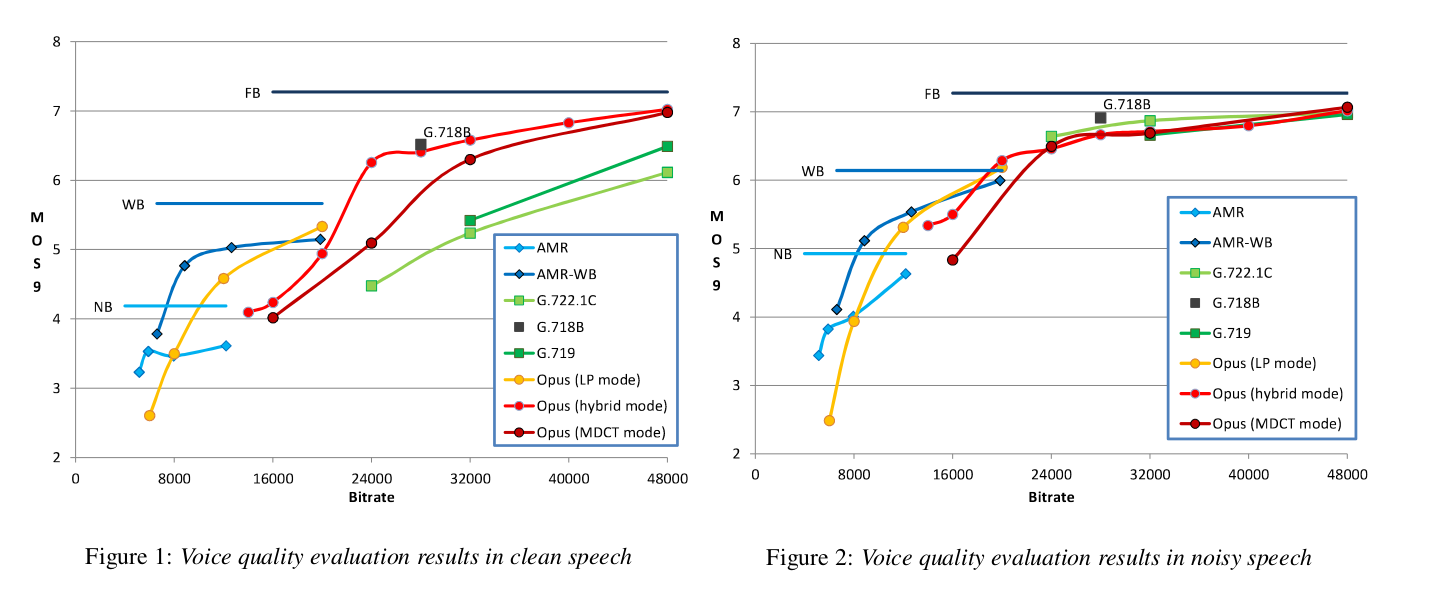
\includegraphics[width=\textwidth]{image.png}
\end{center}

If we choose Codec2 there is little reason to go below 3200bps, as the quality at lower bitrates is not competitive in the modern VoIP landscape, and recordings with background noise or music result in a jumbled mess.

\subsection{Bandwidth}

We should use wide band compression. In most settings it has little impact on the file size, but is a huge gain in audio quality and clarity.

\subsection{Frame size}

%The sweet spot for frame size when encoding speech with LPC is 20ms. It still catches everything someone is saying, even if they are speaking fast. A demonstration of speech encoded with changing frame sizes can be accessed at \href{https://brettpreston.github.io/audio/KnPAudio/frames.wav}{frames.wav}.

Encoding with Opus, frames lengths under 20ms at low bit rates have audible distortions as well as frames sizes over 80ms. This demonstration uses 6VBR wide band, in order to accentuate the distortion: \href{https://brettpreston.github.io/audio/KnPAudio/opusframes.flac}{opus-frames}. In practice, this is a lower bitrate than we would use and so the result would sound better.

\subsection{Algorithm complexity}

The algorithm complexity impacts the processing power required on a device more than it does the file size. In our use case, where we expect the system to be used on modern devices there is no reason not to opt for higher complexity, since it's an easy gain in quality without compromising on the resources that are scarce. The recommendation is complexity 10, unless we expect to work on older mobile devices with a real-time audio stream, in which case we may want to choose 5.


\section{Signal processing, noise reduction and equalizing}

Background noise tends to be an issue with voice recordings, we could implement a noise filter with a small processing footprint, as well as a dynamic range compressor/limiter before encoding the message. This will improve the likelihood of a clear and appropriately loudness balanced audio message.

Noise reduction is recommended pre-encoding for maximum clarity. State-of-the-art noise suppressors tend to be based on neural networks, such as \cite{xiph} \cite{werman}. This is somewhat resource intensive, but not out the question on mobile devices. There is an analysis of XIPH's efficacy and efficiency at \href{https://jmvalin.ca/demo/rnnoise/}{https://jmvalin.ca/demo/rnnoise/}. A demonstration of this process can be found \href{https://brettpreston.github.io/audio/KnPAudio/rnnoise-opus-codec2.flac}{here.}
A potential alternative is an automated Fast Fourier Transform noise suppressor, however, that is likely to involve extensive customization of available tools.

When it comes to Codec2 at 1200bit/s to 3200bit/s, an EQ boost of several decibels at 3kHz is a simple and effective way to improve consonant clarity. Noise suppression and equalizing can make a big difference when making Codec2 viable as demonstrated \href{https://brettpreston.github.io/audio/KnPAudio/voice-denoize-codec2-3kHz-eq-boost.flac}{here.} Compare with the original sample \href{https://brettpreston.github.io/audio/KnPAudio/codec2/deep-voice-noise-3200.c2.flac}{here.} Without these adjustments, Codec2 may not meet the quality expectations of today's users.

%\section{Adjusting the linear predictive coding algorithms}


\section{Recommendations summary}

\begin{itemize}
    \item Before encoding: noise suppression with XIPH or a similar plugin, or a heavily customized Fast Fourier Transform process.
    \item In most use cases, encoding with Opus, 12kbps VBR, mono, wide band, complexity 10, frame size 20ms.\smallskip

    If processing power is scarce, complexity 5.\smallskip

    For extreme file compression, Codec2 3200bps, "Natural" setting. The quality in Codec2 could be improved by widening the band on the higher end. Noise suppression is crucial.
    \item A security conscious decoder such as \cite{symphonia} or \cite{pion}.
    \item After decoding: EQ boost of several decibels at 3kHz, especially with Codec2.
\end{itemize}



\section*{Acknowledgments}
Special thanks to EJ Infeld for help with formatting and editing this analysis, as well as providing valuable context about Mixnets, and to the Wau Holland Foundation for funding this work.


\bibliographystyle{unsrt}
\bibliography{references}
\end{document}

\section{Towards voice anonymization}

In today's world it would be dishonest to claim one can easily anonymize a message and still convey its meaning. Powerful analysis can make non-trivial guesses as to who is speaking based on as little as the words we use. And so without equally powerful methods of anonymization, such as perhaps a large language model rephrasing the message \cite{meyer1}
\cite{meyer2}, there is only so much we can do.

A straightforward way to lose most information other than the words spoken is converting a message with a speech-to-text engine, and then back to speech. This may still carry some unwanted information, as it can  unexpectedly encode artifacts of a person's speech. It is also somewhat process-intensive, and a user who would like to avail themselves of such a system may as well consider sending the message as text. 

Many modern academic attempts at voice anonymization rely heavily on neural network technology \cite{turner2022im} \cite{conversion} but retain the linguistic content of the message. One may propose that this would have a similar efficacy as other resource-intensive methods, such as re-synthesizing the message from text. A fun way to do something roughly equivalent, that may be attractive to users, would be to use one of the popular tools to change one's voice in real-time to that of a celebrity \cite{change}.

We would like to consider whether we can provide some deniability at little computational cost. We can make adjustments to the encoding itself. We can manipulate how LPC encodes speech to achieve voice masking effects at low processing cost and file size. For example, we can make the carrier tone more extreme as it over predicts pitch modulation, or we can make it monotone. \cite{lpc} \cite{knector} We can remove the tone leaving only the noise, or we can remove the noise leaving only the tone. We can adjust the frame size or reduce the bit rate in order to lose distinguishing features of the sound. A demonstration of all of these operations can be heard here: \href{https://brettpreston.github.io/audio/KnPAudio/BP-LPC-Voice-Mask-Demo.mp3}{LPC-Voice-Mask-Demo}. One can somewhat verify the efficacy of this kind of masking by feeding such a sample back into a powerful neural network-based decoder for reconstruction \cite{wavenet}, and if the reconstruction does not sound like the original speaker we could consider that a partial success. Many academic attempts at voice anonymization so far have been in a similar vein - they reduce the information carried by the encoding in one way or another, with varying efficacy. However, one needs to verify that these changes are not easy to reverse-engineer. An overview of some of those attempts, as well as some evaluation can be found in \cite{thesis}. 